\section{Méthodologie}

\subsection{Sélection des génotypes}
Afin d'élargir la portée des expériences, il a été décidé de travailler sur plusieurs variétés.
Les génotypes ont été sélectionnés sur base des variétés testées précédemment par le centre indépendant de promotion fourragère (CIPF).
Les six variétés échantillonnées correspondent à celles qui ont été testées, au minimum l'année précédente et l'année en cours (à savoir 2021 et 2022).
Ce choix confère plusieurs avantages :
\begin{itemize}
    \item Premièrement, les résultats des précédentes cultures réalisées et analysées par le CIPF offrent des informations sur les parties aériennes des six variétés considérées sur au moins deux années consécutives.
    \item Ensuite, les cultures de 2022 ayant été récoltées en septembre, il a été possible de récupérer des échantillons racinaires de cette culture, offrant ainsi des échantillons de fin de culture.
\end{itemize}
Ces six génotypes étudiés sont repris dans le tableau \ref{tab:variete} ci-dessous ainsi que l'identifiant attribué à ces génotypes qui sera par la suite utilisé pour différencier les échantillons.

\begin{table}[ht]
    \centering
    \caption{Génotypes}
    \begin{tabular}{c c c}
        \hline
        \textbf{Identifiant} & \textbf{Variété} & \textbf{Type} \\
        \hline
        \hline
        A & Amiggo & Sorgho fourrager monocoupe \\
        B & RGT Biggben & Sorgho fourrager monocoupe \\
        H & ES Hyperion & Sorgho fourrager monocoupe \\
        J & KWS Juno & Sorgho fourrager monocoupe \\
        S & RGT Swingg & Sorgho fourrager monocoupe \\
        V & Vegga & Sorgho fourrager monocoupe
    \end{tabular}
    \label{tab:variete}
\end{table}

\subsection{Parties aériennes}
Les données des parties aériennes proviennent des rapports d'expériences partagés par le CIPF \citep{cipf_resultats_2021,cipf_resultats_2022}.
Ces rapports reprennent plusieurs informations :
\begin{itemize}
    \item Protocole expérimental : densité de semis, date de culture, culture précédente, fumure, traitement des semences, ...
    \item Des données météorologiques : pluviométrie, température, ...
    \item Les résultats de culture : \% de masse sèche (MS), rendement MS, \% de levée, hauteur des plants, valeur alimentaire, ...
\end{itemize}
Certains résultats de ces rapports ont été récupérés et rassemblés dans un document Excel pour permettre leur utilisation avec le langage de programmation R.

\subsection{Échantillons racinaires}

Les dates de culture de sorgho ainsi que les difficultés expérimentales décrites précédemment ont rendu nécessaire l'obtention d'échantillons de différentes façons.
D'une part, des échantillons racinaires de fin de culture ont été récoltés suite aux tests de cultures réalisés par le CIPF. 
Il s'agit donc de plants de sorgho ayant été cultivé du 17 mai au 21 septembre 2022 et en champ.
D'autre part, des résultats de début de culture sont récupérés via une expérience réalisée en serre et sur une période bien plus courte d'une vingtaine de jour (du 3 avril au 24 avril 2023).
Tous les échantillons racinaires ont été numérisés à l'aide du scanner Epson Perfection V850 Pro.
Les scans ont été faits avec la configuration disponible en annexe \ref{an:config}.

\subsubsection{Échantillons en fin de culture}

\begin{minipage}{0.4\linewidth}
\captionsetup{type=figure,hypcap=true}
\centering
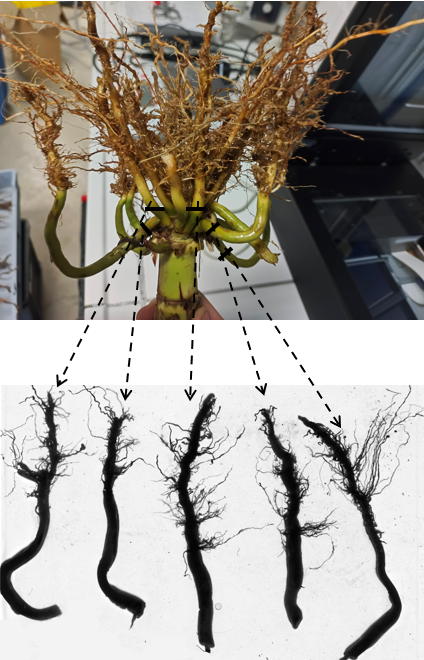
\includegraphics[width=0.65\linewidth]{Image/scan.png}
\captionof{figure}{Numérisation des échantillons racinaires en champs}
\label{fig:scan}
\end{minipage}\hfill
\begin{minipage}{0.5\linewidth}
Les données de fin de culture sont récupérées sur des échantillons racinaires résultant des tests réalisés par le CIPF.
Un résumé du protocole de culture respecté par le CIPF lors de leurs tests de culture de sorgho est disponible en annexe \ref{an:protocole_CIPF}.
Suite à la récolte des parties aériennes, quatre systèmes racinaires de plants de sorgho ont été récupérés de façon aléatoire à la bêche en champ pour chacune des six variétés étudiées.
Les 24 systèmes racinaires ont ensuite été conservés dans le bloc de terre extrait en chambre froide jusqu'à ce qu'ils soient nettoyés et numérisés.
Afin de pouvoir scanner ces échantillons, les racines ont été coupées pour permettre de les scanner en plusieurs parties.
L'image \ref{fig:scan} montre un des systèmes racinaires nettoyés ainsi que le résultat de la numérisation d'une partie de celui-ci.
\end{minipage} 
\newline

\subsubsection{Échantillons en début de culture}
Les racines de plants de début de culture ont été échantillonnés à l'aide de rhizotrons dans les serres de l'UCLouvain.
\newline

\textbf{Rhizotron} \\
Un rhizotron est un montage permettant d'observer le développement racinaire ainsi que la prise de mesure précise de l'architecture racinaire de façon non destructrice.
Pratiquement, les rhizotrons ont été construits comme illustré par la figure \ref{fig:rhizotron}.
Une planche en bois sur laquelle se trouve des mousses est remplie d'un substrat au choix.
Une feuille de papier filtre laissant passer la solution nutritive est ensuite placée sur le substrat.
Finalement, une plaque de plexiglas vient fermer le dispositif avec la graine placée entre le papier filtre et la plaque transparente.
La racine est ainsi visible et peut accéder aux nutriments apportés par l'arrosage du substrat à travers le papier filtre.
\newpage

\begin{figure}[ht]
\centering
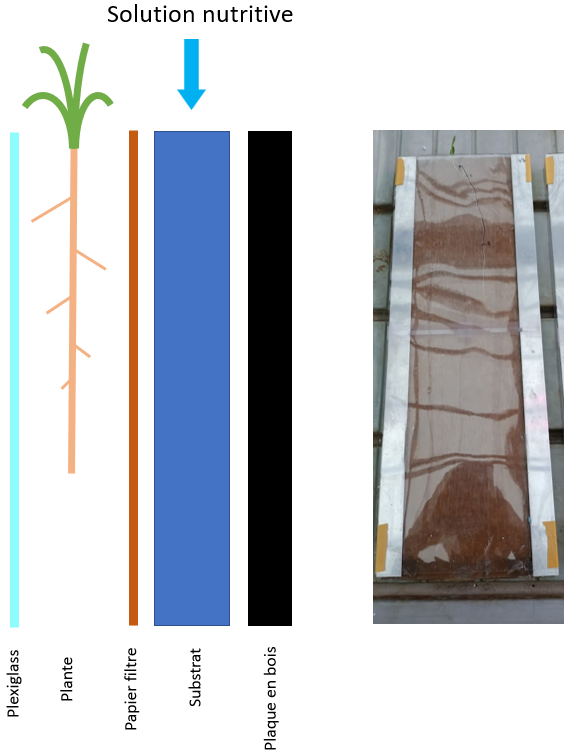
\includegraphics[width=0.5\textwidth]{Image/rhizotron.png}
\caption{Montage d'un rhizotron}
\label{fig:rhizotron}
\end{figure}

Quatre rhizotrons de dimension 60×20 cm ont été réalisés pour chacune des six variétés étudiées faisant un total de 24 rhizotrons contenant chacun un plant de sorgho.
Ceux-ci ont été placés dans la serre 'S.0 27' à l'UCLouvain qui simule un climat tempéré.
Les rhizotrons sont entreposés par six dans des bacs comme montrés en figure \ref{fig:montage}.
Des bouts de polystyrène sont posés au fond des bacs pour permettre l'évacuation de la solution nutritive non absorbée par les racines et empêcher que le bois ne baigne dedans.
La partie du rhizotron laissant apercevoir le système racinaire a systématiquement été placé derrière un autre rhizotron ou derrière une planche pour ceux de devant afin d'éviter une intervention de phototropisme sur les racines.
De plus, les rhizotrons ont été inclinés avec un angle d'environ 30° dans le but de favoriser la croissance de la racine entre le plexiglas et le papier filtre pour que celle-ci reste visible.
\newpage

\begin{figure}[ht]
\centering
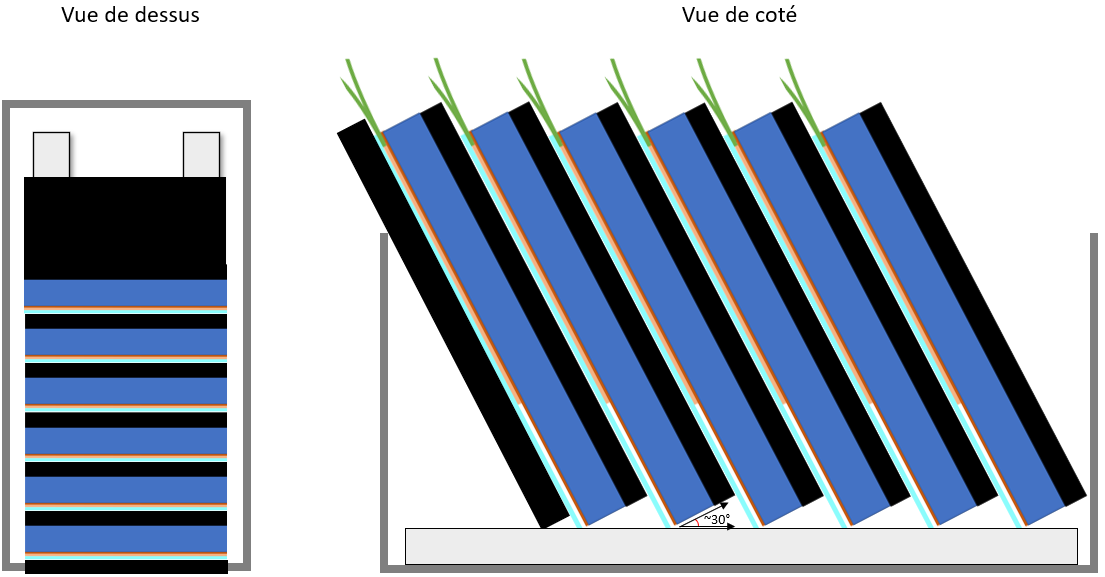
\includegraphics[width=0.75\textwidth]{Image/montage.png}
\caption{Schéma de l'expérience}
\label{fig:montage}
\end{figure}

Le substrat qui est utilisé est de la perlite.
Il s'agit d'un substrat de culture léger, avec une bonne rétention d'eau, ce qui peut favoriser une croissance saine des racines et des plantes.
Chaque rhizotron a été arrosé les lundi, mercredi et vendredi durant toute la durée de l'expérience avec 50 ml de solution de Hoagland.
La solution de Hoagland, dont la composition est reprise en annexe \ref{an:Hoagland}, contient tous les nutriments nécessaires au développement de la majorité des plantes.
Cette fréquence d'arrosage vise à apporter une quantité suffisante d'eau et de nutriment pour permettre aux plantes de se développer sans être exposées à l'un ou l'autre stress.
Un tracé de l'évolution des racines a été effectué de façon régulière afin de pouvoir mesurer des paramètres de croissance.
L'un de ces tracés est disponible en annexe \ref{an:trace}.
\newline

Une première salve de rhizotron s'est avérée être inutilisable dû à la présence de pathogènes dans le dispositif expérimental.
Ceux-ci ont été identifier comme étant des champignons (Stachybotrys echinata et Stachybotrys chartarum).
Une seconde salve a donc été réalisée avec des précautions supplémentaires.
Les échantillons utilisés dans ce travail ont, en conséquence, été traités avec un fongicide (Rovral) une première fois avant le montage des rhizotrons et deux fois supplémentaires au cours de la croissance des plants.
Bien que cela a partiellement réduit l'apparition de champignons, ceux-ci ont malgré tout été observés dans les rhizotrons utilisés et peuvent de ce fait avoir influencé la croissance des plants.

\subsection{Numérisation des échantillons}
L'acquisition des échantillons précédemment décrite permet de quantifier certaines caractéristiques de l'architecture racinaire chez ces six variétés de sorgho.
Certains problèmes évoqués auparavant se présentent pour les deux sets d'échantillons (fin de culture en champs et début de culture en rhizotron).
Les systèmes racinaires en champs sont ceux de plantes ayant terminé leurs croissances et sont alors très importants.
Cela rend les mesures complexes à réaliser car les racines sont assez longues et se chevauchent.
Les racines provenant des rhizotrons permettent quant à elles des mesures précises et temporelles, mais résultent de conditions assez artificielles et ne donnent pas l'état final des racines.
De ce fait, la quantification se fera, compte tenu du paramètre mesuré, sur des échantillons de fin de culture ou de début de culture.

\subsubsection{Smartroot}

\begin{minipage}{0.5\linewidth}
\captionsetup{type=figure,hypcap=true}
\centering
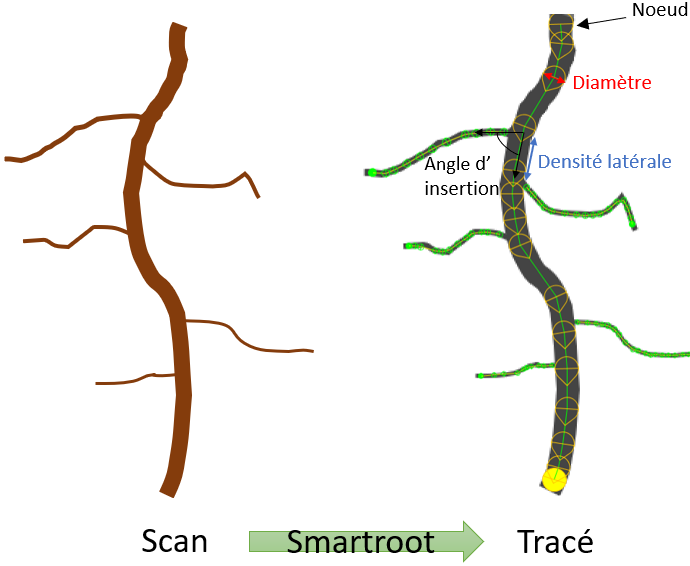
\includegraphics[width=1\linewidth]{Image/schema smartroot.png}
\captionof{figure}{Smartroot}
\label{fig:schema smartroot}
\end{minipage}\hfill
\begin{minipage}{0.45\linewidth}
Toutes les mesures réalisées sur les échantillons racinaires ont été faites à l'aide de Smartroot \citep{lobet_novel_2011}.
Smartroot est un logiciel d'analyse d'images basé sur ImageJ qui permet la quantification de la croissance et d'architecture racinaire complexe.
Cette quantification se fait via le traçage d'image d'échantillon de système racinaire (figure \ref{fig:schema smartroot}).
Les racines sont représentées par un ensemble de points (appelés nœuds) reliés entre eux.
Le logiciel est par la suite capable, sur base des nœuds de fournir des mesures de l'architecture du système racinaire telles que la longueur, le diamètre, la densité de latérale, l'angle d'insertion des latérales, ...
\end{minipage} 
\newline

\noindent Les logiciels d'analyse d'image peuvent être classés en trois catégories :
\begin{itemize}
    \item Manuels : qui ont l'avantage de pouvoir être utilisables dans presque toutes les situations, mais qui requièrent énormément d'interactions et donc de travail pour l'utilisateur.
    \item Automatiques : qui ne fonctionnement souvent que dans des cas très spécifiques adaptés au logiciel, mais qui sont très rapides et demandent peu de travail.
    \item Semi-automatiques : qui utilisent des algorithmes permettant de faciliter et d'accélérer l'analyse d'images à l'aide d'interventions de la part de l'utilisateur pour corriger et orienter les algorithmes.
\end{itemize}
Smartroot a été conçu pour réaliser les tracés racinaires de façon semi-automatique.
Cela permet de considérablement réduire le temps et le nombre d'interactions nécessaires de l'utilisateur tout en restant modulable à bon nombre de situations.

\subsubsection{Structure des données}

Le fichier qui contient le tracé des racines est enregistré en utilisant le format Root System Markup Language (RSML) \citep{lobet_plant_2014}.
Ce format est essentiellement un fichier XML (eXtensible Markup Language) qui contient des informations topologiques, géométriques et autres données numériques qui permettent de capturer la complexité d'un système racinaire (en 2D, 3D et données temporelles).
Le langage XML est largement utilisé pour échanger des données entre des applications hétérogènes, car il est facile à lire et à écrire pour les humains et les machines. 
Il est également extensible, ce qui signifie que les développeurs peuvent définir leurs propres balises pour représenter des données spécifiques à leur application (dans le cas du RSML, des données racinaires).
Une représentation visuelle de la structure d'un fichier RSML est disponible en annexe \ref{an:RSML}.
Smartroot propose par ailleurs la possibilité d'extraire directement les données racinaires plus globales dans un fichier CSV (Comma Separated Values).
Ce fichier contient alors entre autres la longueur, le diamètre moyen, l'angle d'insertion, la direction de chaque racine.
Les analyses descriptives ainsi que l'inférence statistique seront dès lors réalisées sur base de ces fichiers.
\newline

Tous les fichiers de données RSML et CSV résultant de la numérisation des échantillons et de l'utilisation de Smartroot sont disponibles sur \href{https://github.com/ndegives/Memoire}{Github}.
Les échantillons suivent les nomenclatures suivantes :
\begin{itemize}
    \item Parties aériennes : les données moyennes sont simplement organisées à l'aide du nom de la variété.
    \item Les échantillons de fin de culture : chaque racine est nommée comme suit :
    \begin{center} Identifiant variété\_Numéro de plante\_N\oe ud de la racine\_ Racine (e.g. A2\_1\_4) \end{center}
    \item Les échantillons en rhizotron : chaque plant est identifié par l'identifiant de la variété suivi d'un numéro pour identifier le plant au sein de la variété (e.g. S2)
\end{itemize}

\subsection{Modélisation de l'architecture racinaire}

Suite à l'analyse des images provenant des différents échantillons racinaire, il est possible de travailler avec les données chiffrées qui en résultent.
Dans un premier temps, une caractérisation sera faite afin d'identifier les valeurs de certain paramètre d'architecture racinaire propres au sorgho.
Ensuite, des paramètres seront introduits en input d'un modèle afin de reconstruire un système racinaire complet.

\subsubsection{ArchiSimple}

ArchiSimple  \citep{pages_calibration_2014} est un modèle permettant la génération d'ASR.
C'est un modèle dynamique architectural et fonctionnel dans lequel un système racinaire est représenté comme un ensemble de petits segments (quelques millimètres) et de méristèmes.
ArchiSimple estime, à l'aide de cinq processus majeurs, l'évolution d'une ASR.
Ces processus sont : l'émission de racines adventives, l'élongation de racines préexistantes, la ramification, la croissance radiale et l'abscission racinaire.
Chacun de ces processus est quantifié à l'aide des inputs qui sont requis par le modèle.
\newline

Une vingtaine d'inputs est nécessaire au modèle, ceux-ci sont repris dans le tableau \ref{tab:archisimple} ci-dessous.
En fonction de l'input estimé et suite aux difficultés d'échantillonnage et d'analyse décrites précédemment, les données utilisées proviendront soit des racines en début de culture ('début' dans le tableau \ref{tab:archisimple}) soit en fin de culture ('fin' dans le tableau \ref{tab:archisimple}).
Enfin, certains paramètres n'ont pas pu être extraits des données récoltées.
Quelques uns ont pu être quantifiés pour le sorgho sur base de sources bibliographiques.
Les derniers paramètres, qui n'ont pas pu être quantifiés pour le sorgho, sont alors alignés sur base de paramètres génériques identifiés pour les monocotylédones par \cite{gerard_modelling_2017} et disponibles en annexe \ref{an:Poaceae} ('monocot' dans le tableau \ref{tab:archisimple}).

\newpage 

\begin{table}[ht]
    \centering
    \caption{Paramètres de ArchiSimple et sources pour leurs estimations}
    \begin{tabular}{p{7.5cm}|p{2.2cm}|p{3.2cm}|p{3cm}}
        Paramètre & Abréviation & Unité & Source \\
        \hline
        Durée de simulation & $simtime$ & $jour$ & / \\
        Vitesse d'émission de racines séminales & $erSem$ & $jour^{-1}$ & Début \\
        Diamètre relatif séminale (p/r à Dmax) & $dSem$ & / & Début \\
        Nombre maximum de séminale & $maxSem$ & / & Début \\
        Âge de commencement d'émission de racines adventives & $ageAdv$ & $jour$ & \cite{chantereau_sorgho_2013} \\
        Distance avant racines adventives & $distAdv$ & $mm$ & Début \\
        Taux d'émission racines adventives & $erAdv$ & $jour^{-1}$ & \cite{kumar_goyal_how_2021} \\
        Diamètre relatif adventive (p/r à Dmax) & $dAdv$ & / & Fin \\
        Nombre maximal de racines adventives & $maxAdv$ & / & Fin \\
        Diamètre minimum & $D_{min}$ & $mm$ & Fin \\
        Diamètre maximum & $D_{max}$ & $mm$ & Fin \\
        Pente de la relation entre vitesse de croissance et diamètre & $EL$ & $mm.mm^{-1}.day^{-1}$ & Début \\
        Type de tropisme (0: plagio; -1: geo-; +1: geo+; 2: exo) & $TrT$ & / & monocot \\
        Intensité du tropisme & $TrInt$ & / & monocot \\
        Durée de développement des primordium & $PDT$ & $day$ & monocot \\
        Distance inter-primordium & $IPD$ & $mm$ & Début \\
        Probabilité d'émergence à $D_{max}$ & $pdmax$ & / & / \\
        Probabilité d'émergence à $D_{min}$ & $pdmin$ & / & / \\
        Ratio entre diamètres mère-fille & $RDM$ & / & Fin \\
        Coefficient de variation des latérales & $CVDD$ & / & Fin \\
        Masse volumique de tissus racinaire & $TMD$ & $g.cm^3$ & \cite{lamb_bioenergy_2022} \\
        Coefficient de durée de croissance & $GDs$ & $day.mm^{-2}$ & monocot \\
        Coefficient de croissance radiale & $SGC$ & / & monocot  \\
        Coefficient de durée de vie & $LDC$ & $Jour.mm.mg^{-1}$ & monocot
    \end{tabular}
    \label{tab:archisimple}
\end{table}

À chaque pas de temps (d'un jour), le système racinaire évolue sur base de ces paramètres fournis en input en suivant des règles qui définissent l'intensité des principaux processus de développement :

\begin{itemize}
    \item \textbf{Émission de racines adventives :} 
    L'émission de racines adventives est supposée constante en fonction du temps, jusqu'à ce que le nombre maximal de racines adventives soit atteint.
    Ce processus est particulièrement important dans le cas du sorgho étant donné que ces racines adventives constituent une partie très importante de son système racinaire.
    Les racines sont émises avec un diamètre pour leur apex qui définira leur croissance.
    \item \textbf{Élongation des racines préexistantes :}
    L'élongation d'une racine est enclenchée après le stade primordial qui est fixé à cinq jours.
    Le taux d'élongation potentiel (PER) dépend grandement du diamètre de l'apex et est défini par les équations suivantes :
    \begin{equation}
    PER = 
    \begin{cases}
    EL*D & \text{si } D>D_{min} \text{ et } Age < GD \\
    0 & \text{si } D \leq D_{min} \text{ ou } Age \geq GD
    \end{cases}
    \label{eq:PER}
    \end{equation}
    La durée de croissance (Growth duration : GD) est lui-même également construit sur base du diamètre via l'équation :
    \begin{equation} GD=GD_s*D^2 \end{equation}
    $GD_s$ étant alors un paramètre de durée de croissance [$day*mm^{-2}$].
    La trajectoire empruntée par les racines est calculée sur base de : la direction initiale, une perturbation aléatoire et le type et coefficient de tropisme (TrT et TrInt).
    Cela permet de simuler les contraintes mécaniques présentent dans le sol ainsi que le gravitropisme (influence verticale due à la gravité) ou le plagiotropisme (influence horizontale due à la répartition d'auxine suivant la gravité).
    \item \textbf{Ramification :} 
    Les ramifications sont générées de façon acropétale (de la base vers l'apex) et sont espacées de façon régulière sur base de la distance entre primordium (inter-primordium distance : IPD).
    Le diamètre de chaque latérale est défini aléatoirement au sein d'une distribution normale dont la moyenne est le diamètre de la racine parente multipliée par le paramètre RDM et l'écart-type est le produit de cette moyenne et du paramètre de variation CVDD.
    \item \textbf{Croissance radiale :}
    L'estimation de celle-ci suit le raisonnement suivant :
    chaque racine contribue à la croissance radiale des racines auxquelles elle est connectée, en fonction de sa propre section transversale, dès qu'elle commence à s'allonger. 
    Le coefficient de proportionnalité est le paramètre de modèle SGC, qui est proche de 1 pour plusieurs espèces.
    Dans le cas des monocotylédones comme le sorgho, ce paramètre est fixé à 0 étant donné que ces plantes ne présente pas de croissance radiale.
    \item \textbf{Sénescence et Abscission :}
    La sénescence d'une racine débute lorsque la durée après la fin de sa croissance dépasse son temps de vie (life duration : LD).
    Ce temps de vie dépend à nouveau du diamètre et est défini par l'équation suivante :
    \begin{equation} 
    LD=LDC*D^2*RTD 
    \label{eq:LD}
    \end{equation}
    ou $LDC$ et $RTD$ sont des paramètres du modèle.
    Une racine morte reste présente tant qu'une de ses latérales est encore vivante et ne se détache donc que lorsque toutes les latérales ont excédées leurs durées de vies.
    Les différents facteurs environnementaux pouvant affect la durée de vie des racines ne sont dans ce cas pas pris en compte dans ce modèle.
\end{itemize}

ArchiSimple se différencie fortement des autres modèles par la simplicité qu'il conserve.
Les différents types racinaires sont volontairement ignorés dès lors que ceux-ci ne sont pas basés sur la physiologie des racines.
À la place, le modèle se base sur des relations explicites telles que le paramètre qui met en relation le taux d'élongation potentiel avec le diamètre.
Le diamètre racinaire occupe alors une place centrale dans ce modèle étant donné que seul le diamètre des méristèmes est utilisé pour décrire les capacités de développement propre à chaque racine.

\subsubsection{Caractérisation de l'ASR, les principaux paramètres}

Afin d'estimer les différents paramètres nécessaires en input de ArchiSimple, des statistiques descriptives ainsi que de l'inférence sont réalisées sur les données provenant des échantillons.
Tous les traitements de données, tracés et analyses sont réalisées à l'aide du logiciel R (4.2.2).
L'élimination d'outlier est réalisé à l'aide de la méthode IQR (interquartile range).
Les modèles linéaires sont construits avec la fonction lm() et les analyse de variances avec la fonction anova() pour tester les effets des différentes variétés sur les traits architecturaux.
Les variétés sont considérées comme facteur fixe et le niveau de confiance utilisé pour les tests statistiques est fixé à : $\alpha$ = 0.05.
Les hypothèses sous-jacentes à l'utilisation d'un modèle ANOVA (normalité, indépendance et égalité des variances) sont vérifiées pour chacun des modèles utilisés.
\newline

\cite{pages_calibration_2014,wu_relationships_2016,pages_seeking_2018} ont proposé et étudiés un set de cinq paramètres qui permettent une bonne caractérisation de l'ASR.
Ces cinq traits font partie ou découle des inputs de 'ArchiSimple' et ils offrent une vision assez complète de l'architecture racinaire.
Ces cinq paramètres sont :
\begin{itemize}
    \item \textbf{Le diamètre minimal, Dmin : } reflète la finesse des nombreuses racines fines qui ont une fonction purement absorbante \citep{pages_seeking_2018}.
    Développer des racines de fin diamètres est une stratégie permettant d'augmenter la surface d'échange sol-racines à un coût minimum.
    Afin d'estimer ce paramètre, le diamètre de la racine latérale la plus fine pour chaque racine nodale en fin de culture est récupérée.
    L'estimation de Dmin est alors estimé sur base d'un modèle ANOVA réalisé sur les distributions de ces plus fins diamètres en fonction de la variété.
    \item \textbf{Le diamètre maximal, Dmax : } est souvent observé sur les racines les plus longues et offre différents avantages.
    Un plus grand diamètre est généralement corrélé avec une meilleure exploration des sols.
    Dmax correspond au maximum de la distribution des diamètres des racines nodales récupérées, pour chaque variété, sur les plants échantillonnés en fin de culture.
    \item \textbf{L'étendue des diamètres, Drange :} possède également un impact sur le volume de sol colonisé.
    En effet, \cite{pages_links_2011} a montré qu'une plus grande variabilité entre les diamètres extrêmes est positivement corrélée avec une plus grande portée des racines.
    Drange est alors calculé sur base des diamètres extrêmes comme $2*(D_{max}-D_{min})/(D_{max}+D_{min})$ pour chaque racine nodales et ses latérales.
    \item \textbf{La distance entre latérale, IBD : } est l'inverse de la densité de latérales.
    Ce paramètre définit donc la densité des racines dans le sol et ainsi leur exploration du sol.
    IBD est mesuré à l'aide de la distance moyenne entre deux latérales voisines sur la même racine parente.
    La distance entre latérales est considérée équivalente à la distance entre primordium dès lors que l'on considère que chaque primordium mène à la formation d'une latérale.
    IBD correspond donc à IPD dans ArchiSimple.
    \item \textbf{La pente de la relation linéaire entre le diamètre d'une latérale et le diamètre de sa racine mère, DIDm : } représente l'évolution du diamètre de latérales en fonction du diamètre de la racine parente.
    Il est estimé sur base de la pente de la régression linéaire sur les diamètres de racines fille en fonction de la racine parente.
    Cette estimation de la relation entre racines fille/mère correspond au paramètre RDM de ArchiSimple. 
\end{itemize}

Ces traits permettent de capturer l'essentiel de la capacité d'un système racinaire à explorer et à exploiter les sols.
Il a également été observé que ces traits sont majoritairement influencés par l'espèce de plante et en moindre mesure par l'environnement les rendant ainsi particulièrement adaptés pour établir les différences d'ASR entre différentes espèces voir variétés.
Ceux-ci bénéficieront donc, dans un premier temps, d'un développement statistique plus approfondi afin d'identifier des similitudes ou des différences entre les six variétés échantillonnées.
\newline

Le paramètre EL n'est pas repris dans ces cinq paramètres, mais occupe aussi un rôle primordial dans ArchiSimple.
Celui-ci correspond à la relation linéaire qu'il y a entre le diamètre d'une racine et la croissance racinaire.
L'estimation de celui-ci a donc un impact sur l'allure générale du système généré par ArchiSimple.
Ce paramètre, avec le diamètre des racines primaires, sont les raisons qui ont nécessité de faire des tests en rhizotron afin de quantifier la croissance racinaire.
EL est estimé comme la pente de la régression linéaire de la vitesse de croissance en fonction du diamètre.
Le résultat obtenu sur les racines primaires sera ensuite généralisé à l'ensemble du système racinaire.